\begin{figure}[h!]
    \centering
    \caption{Distributions of estimated landlord shares and counterfactual 
                changes in rents and total wages, urban ZIP codes}
    \label{fig:cf_hist_rents_wages_shares}

    \begin{subfigure}{0.65\textwidth}
        \caption*{Landlord share}
        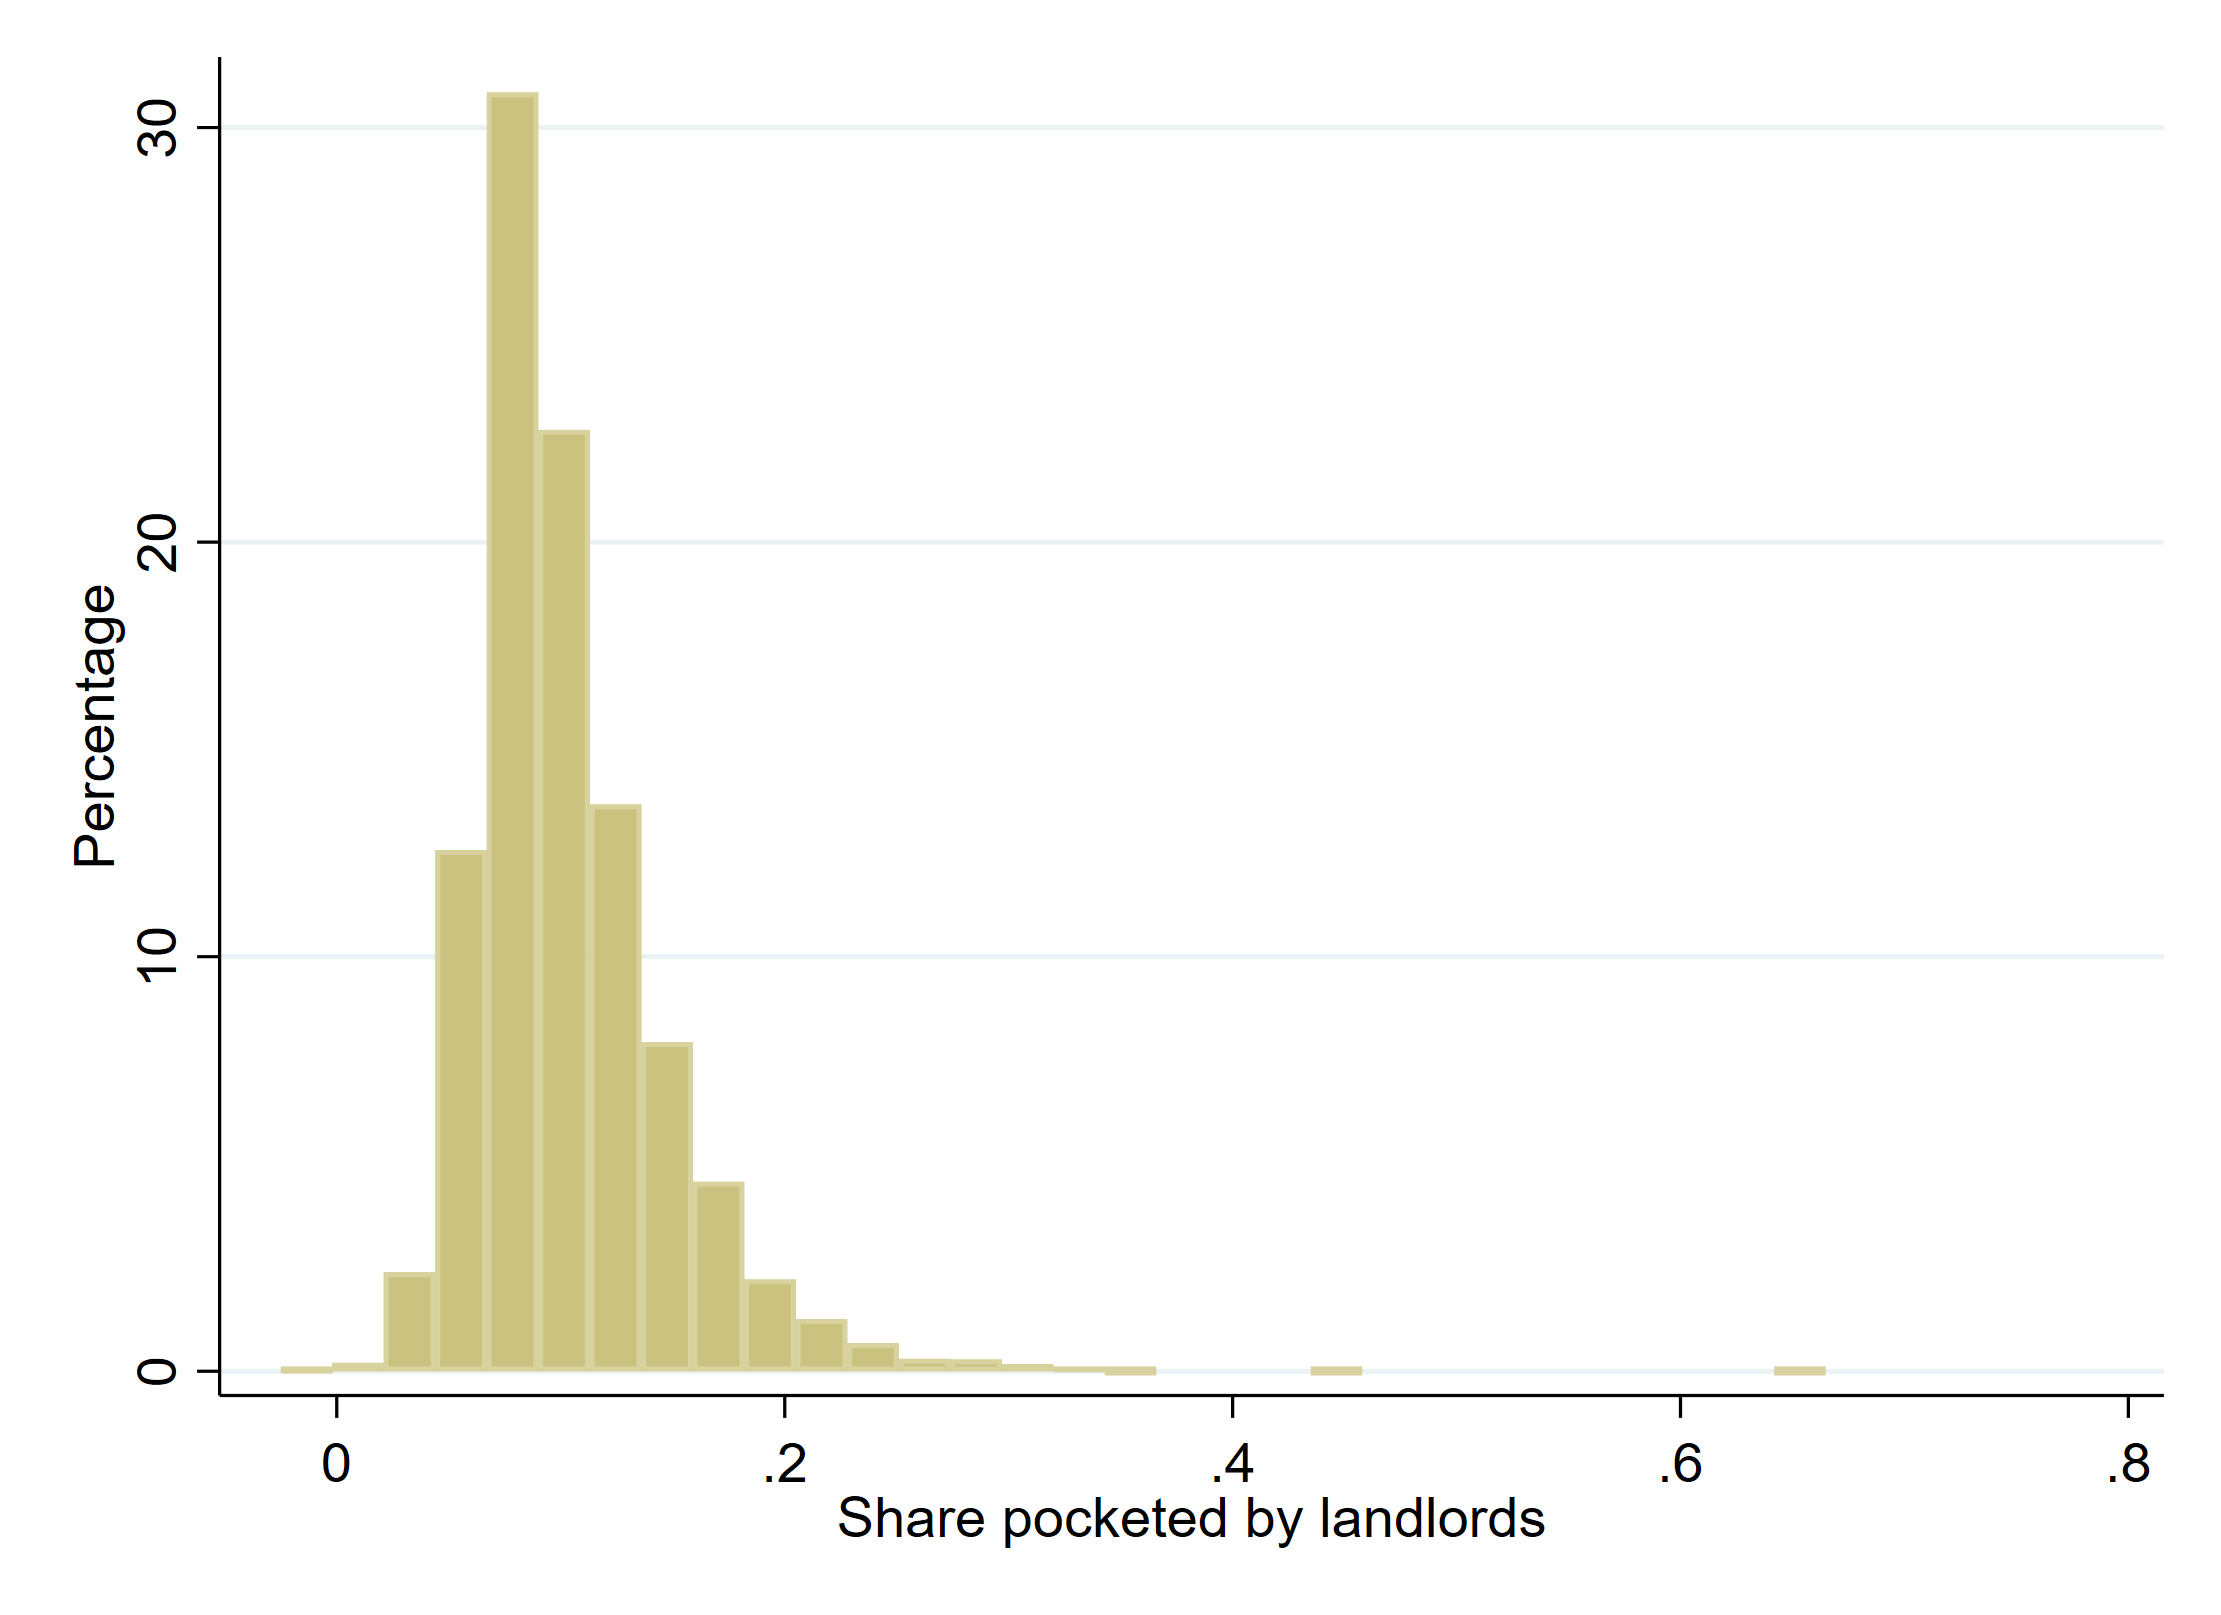
\includegraphics[width = 1\textwidth]{counterfactuals/output/hist_rho.png}
    \end{subfigure}\\
    \begin{subfigure}{0.5\textwidth}
        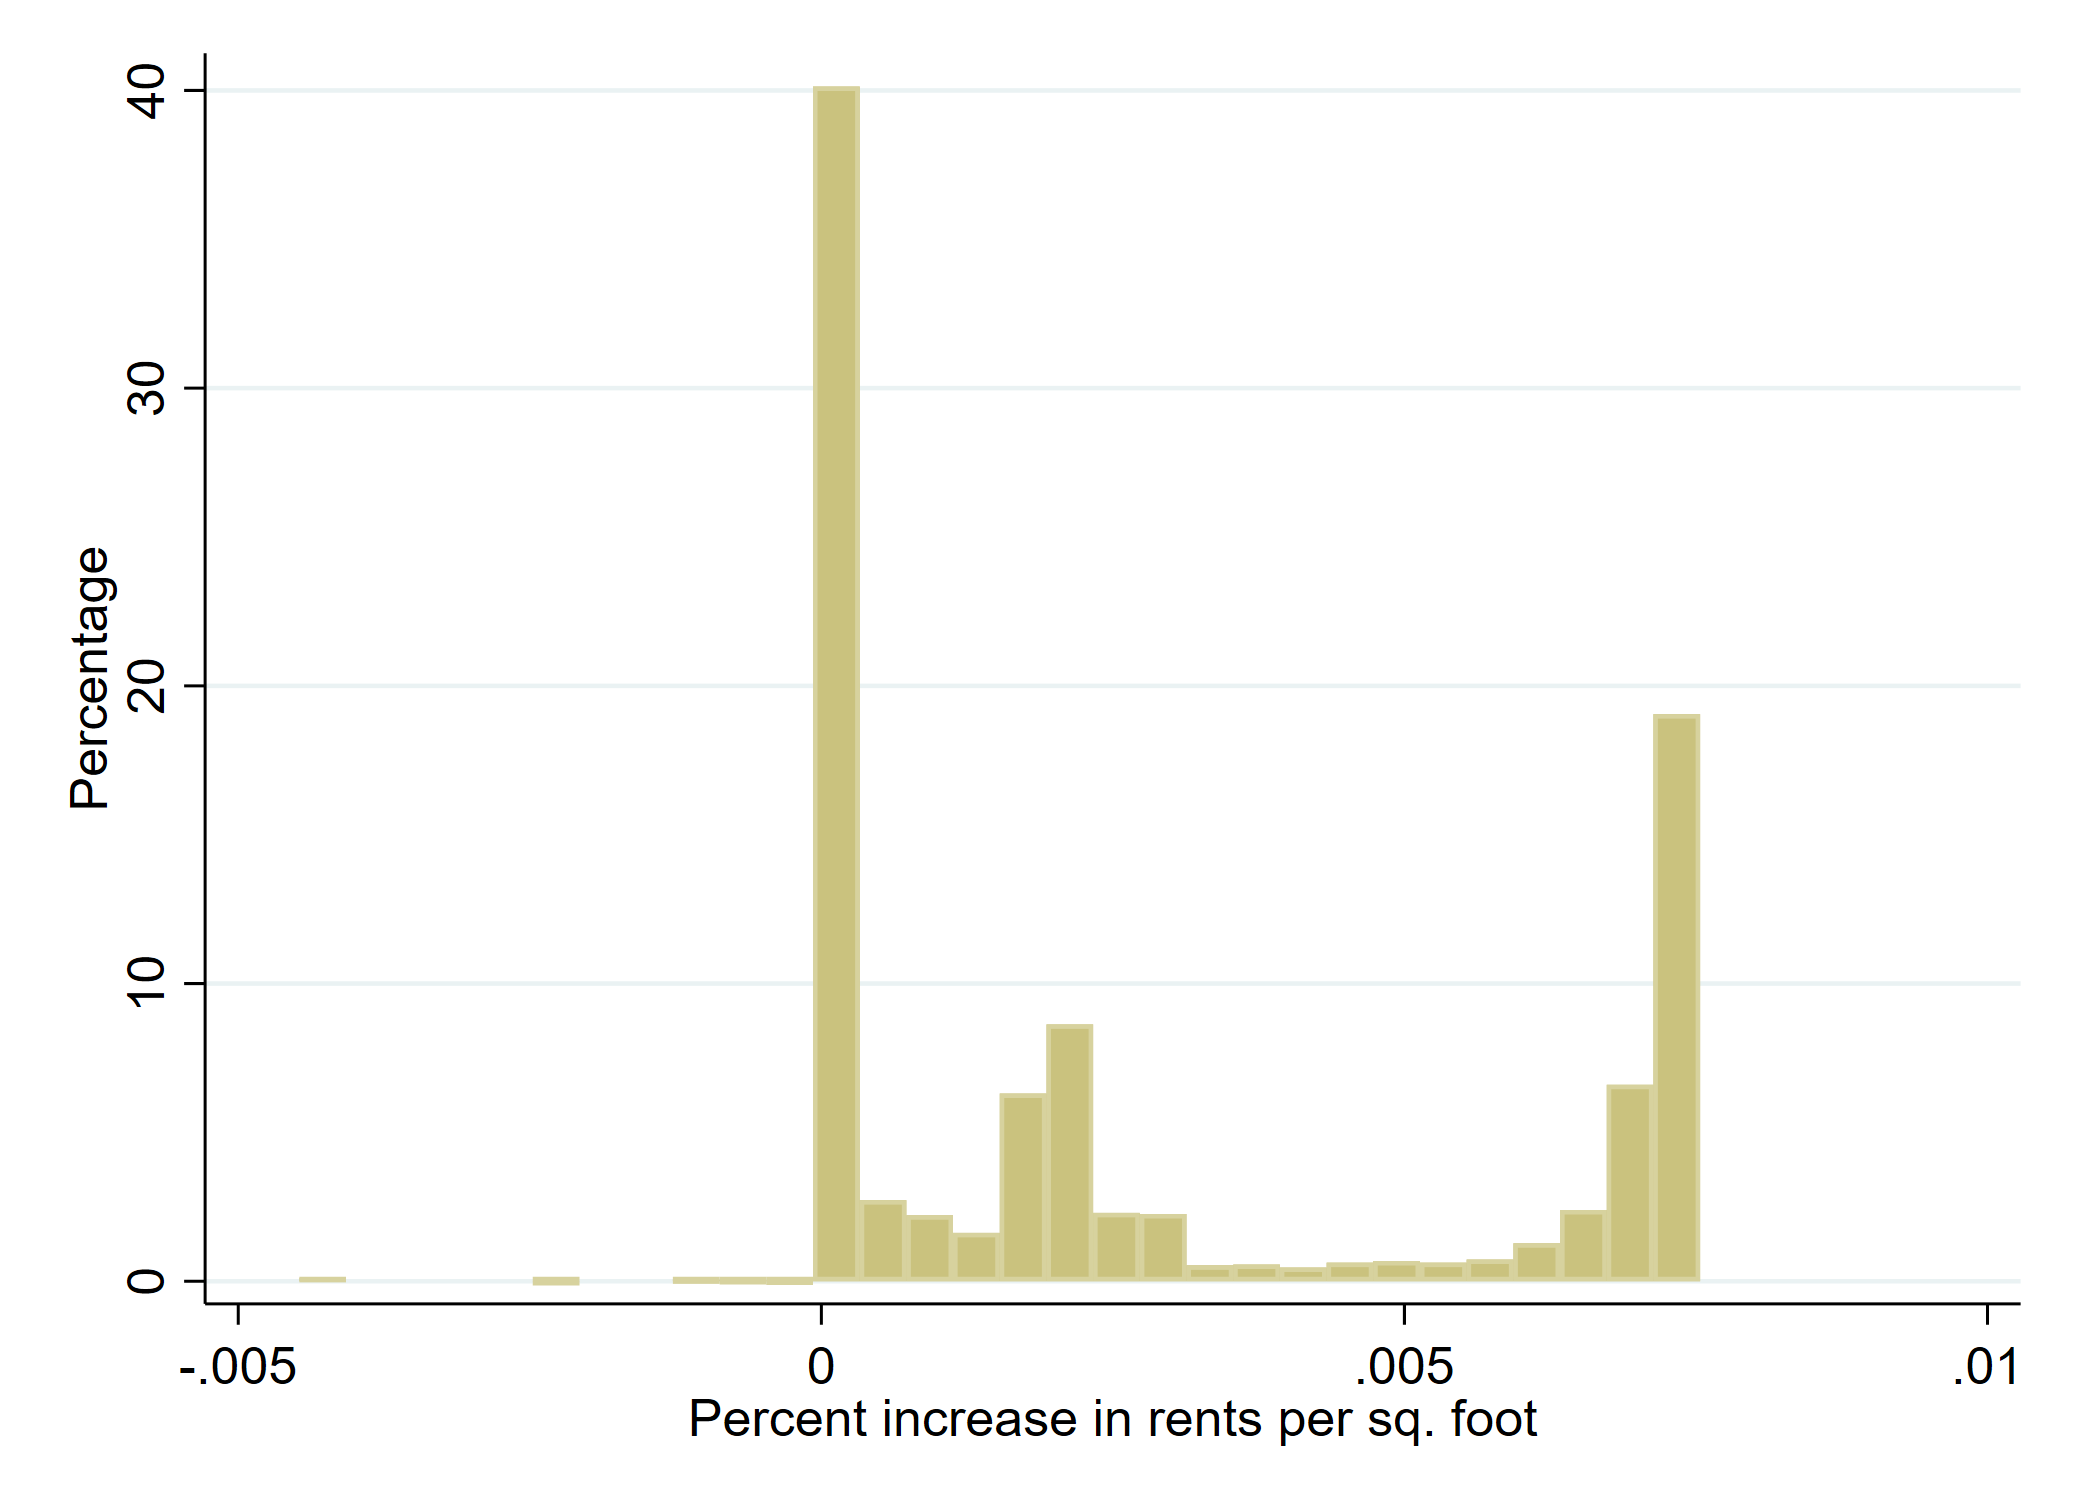
\includegraphics[width = .95\textwidth]{counterfactuals/output/hist_perc_incr_rent.png}
        \caption*{Log(rents)}
    \end{subfigure}%
    \begin{subfigure}{0.5\textwidth}
        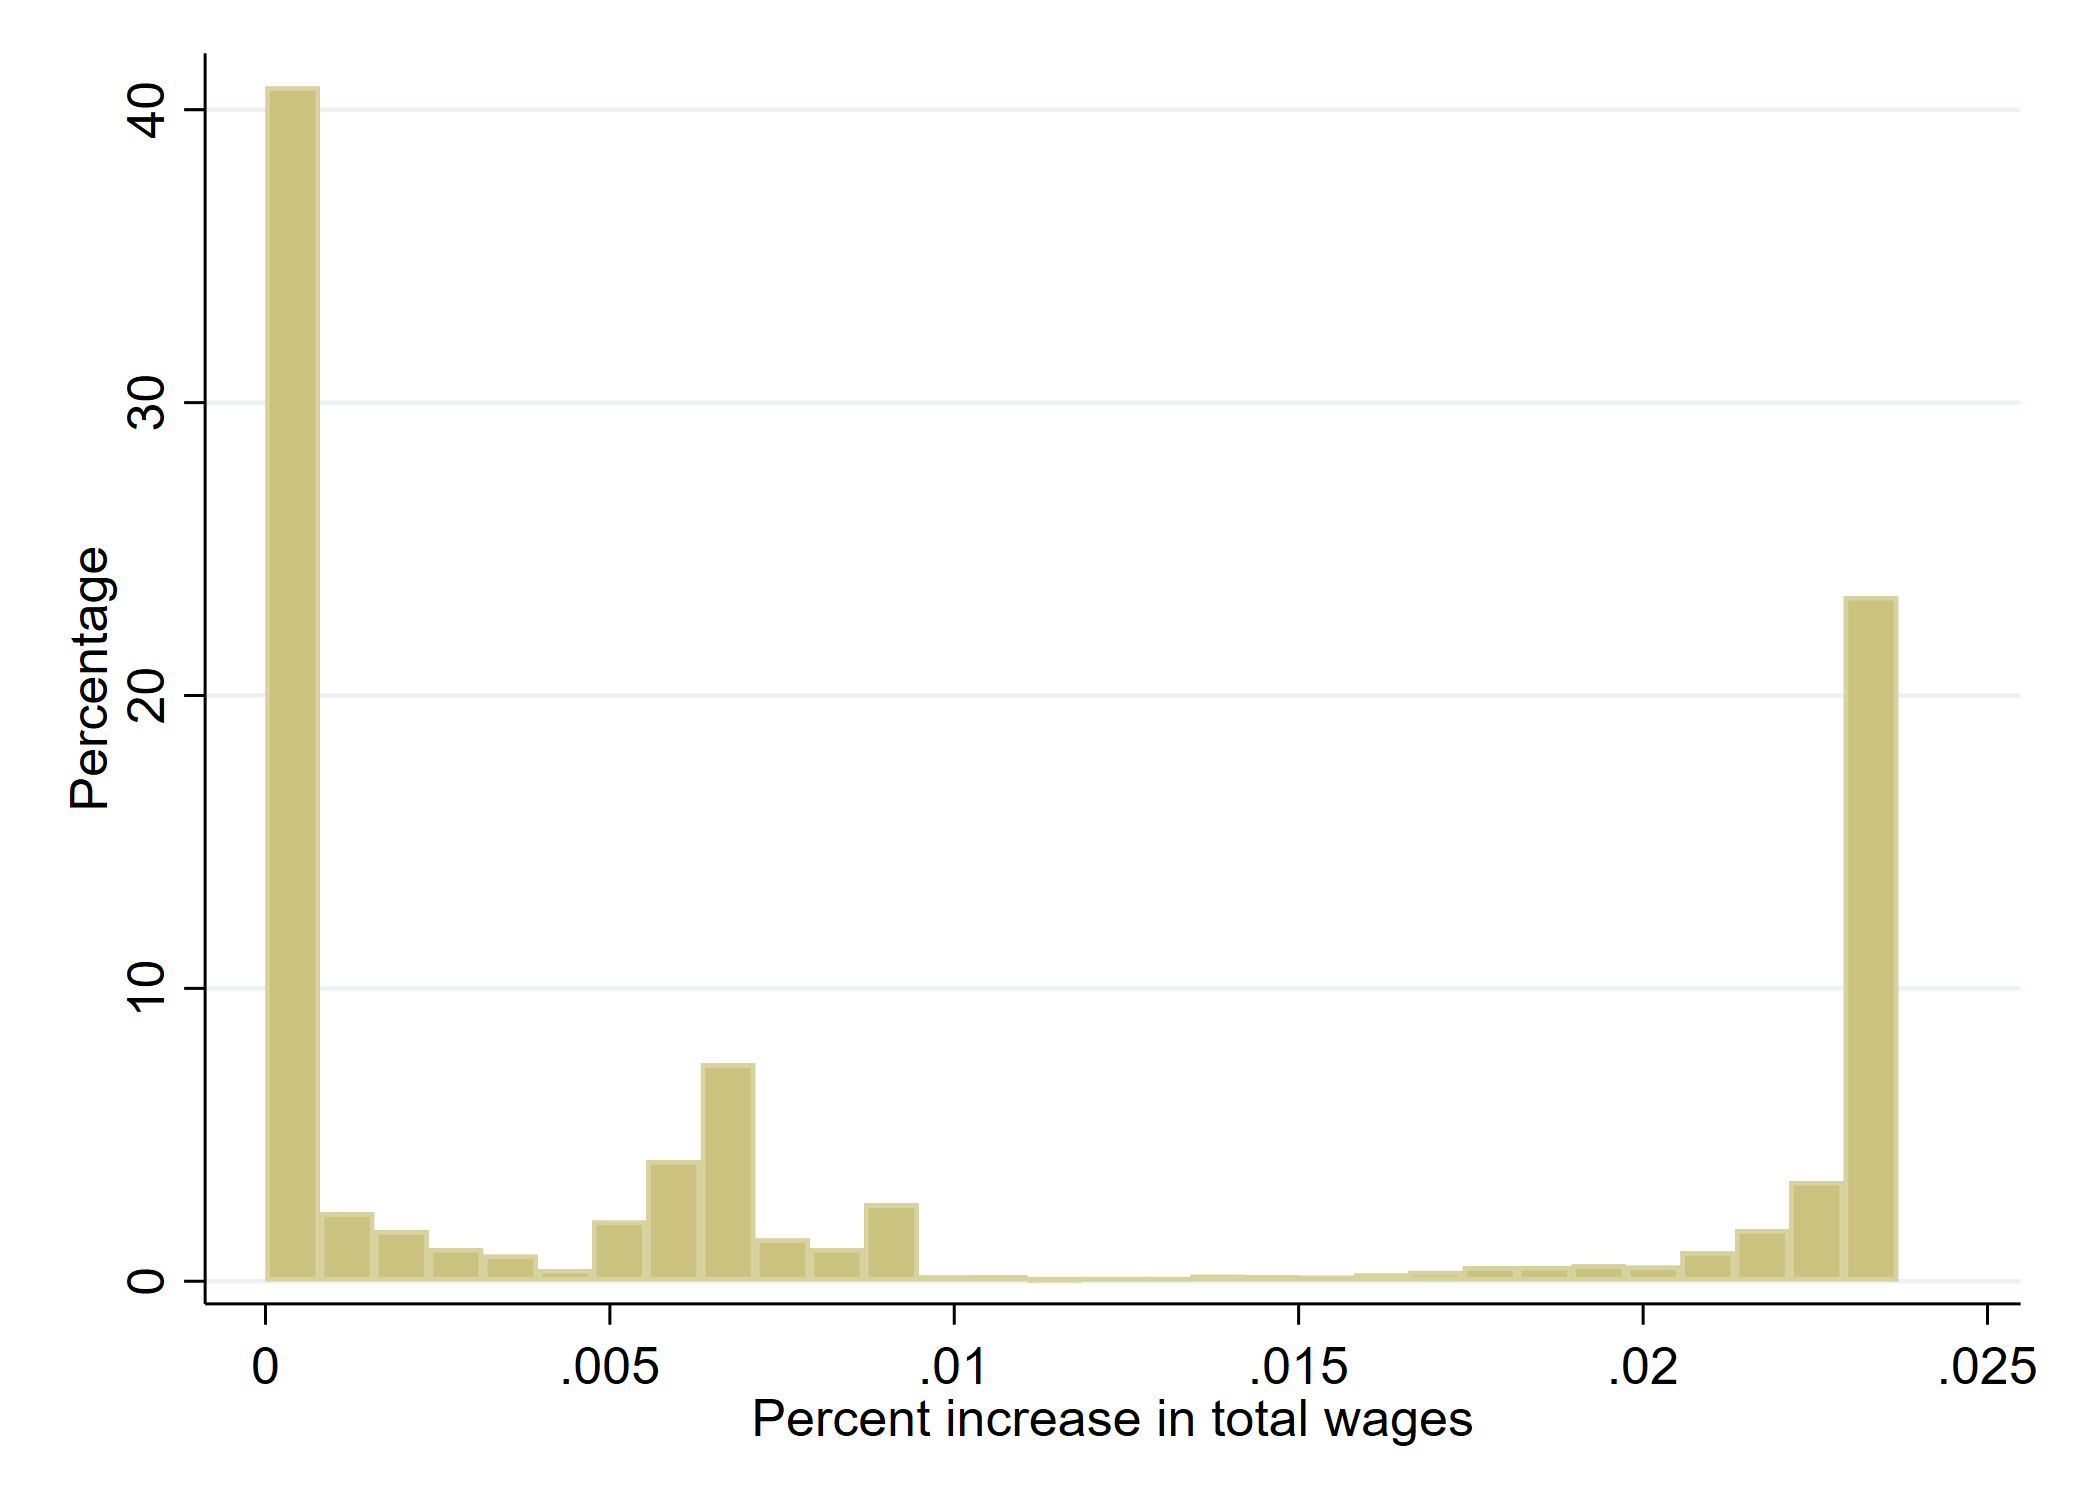
\includegraphics[width = .95\textwidth]{counterfactuals/output/hist_perc_incr_wagebill.png}
        \caption*{Log(total wages)}
    \end{subfigure}

    \begin{minipage}{.95\textwidth} \footnotesize
        \vspace{3mm}
        Notes: 
        Data are from the LODES and the minimum wage panel described in Section 
        \ref{sec:mw_construction}.
        The figures show the distribution of estimated landlord shares in 
        panel (a), estimated changes in log rents in panel (b) and 
        estimated changes in log total wages in panel (c),
        generated by a counterfactual increase to \$9 in the federal MW in 
        January 2020, holding constant other MW policies in their December 2019 
        levels.
        The unit of observation is the urban ZIP code, where we define a ZIP code 
        as urban if at least 80\% of its population is classified as urban by
        the 2010 Census.
        The landlord share is defined as the ratio between the increase in rents
        and the increase in total wages multipled by the share of housing 
        expenditure in the ZIP code, assumed to be 0.35 for all ZIP codes.
    \end{minipage}
\end{figure}
